\ifx\wholebook\relax \else

\documentclass[b5paper]{article}
\usepackage[nomarginpar
  %, margin=.5in
]{geometry}

\addtolength{\oddsidemargin}{-0.05in}
\addtolength{\evensidemargin}{-0.05in}
\addtolength{\textwidth}{0.1in}
\usepackage[en]{../../prelude}

\setcounter{page}{1}

\begin{document}

\title{Selection sort}

\author{Xinyu LIU
\thanks{{\bfseries Xinyu LIU} \newline
  Email: liuxinyu95@gmail.com \newline}
  }

\maketitle
\fi

\markboth{Selection sort}{Elementary Algorithms}

\ifx\wholebook\relax
\chapter{Selection sort}
\numberwithin{Exercise}{chapter}
\fi

\lstset{frame = single}
\label{introduction} \index{selection sort}
Selection sort is a straightforward sorting algorithm. It repeatedly selects the minimum (or maximum) from a collection of elements. The performance is below the divide and conqueror algorithms, like quick sort and merge sort. We'll seek varies of improvement and finally evolve it to heap sort, achieving $O(n \lg n)$ time bound, the upper limit of comparison based sort algorithms.

When facing a bunch of grapes, there are two types of people. One love to pick the biggest grape every time, the other always pick the smallest one. The former enjoy the grape in ascending order of size, while the latter in descending order. In either case, one essentially applies selection sort method, defined as:

\begin{enumerate}
\item If the collection is empty, the sorted result is empty;
\item Otherwise, select the minimum element, and append it to the sorted result.
\end{enumerate}

It sorts elements in ascending order as shown in \cref{fig:sel-sort}. If select the maximum, then it sorts in descending order. The compare operation can be abstract.

\be
\begin{array}{rcl}
sort\ [\ ]  & = & [\ ] \\
sort\ A & = & m : sort\ (A - [m]) \quad \text{where}\ m = \min\ A
\end{array}
\ee

$A - [m]$ means the remaining elements in $A$ except $m$. The corresponding imperative implementation is as below:

\begin{algorithmic}[1]
\Function{Sort}{$A$}
  \State $X \gets [\ ]$
  \While{$A \neq [\ ]$}
    \State $x \gets$ \Call{Min}{$A$}
    \State \Call{Del}{$A, x$}
    \State \Call{Append}{$X, x$}
  \EndWhile
  \State \Return $X$
\EndFunction
\end{algorithmic}

\begin{figure}[htbp]
  \centering
  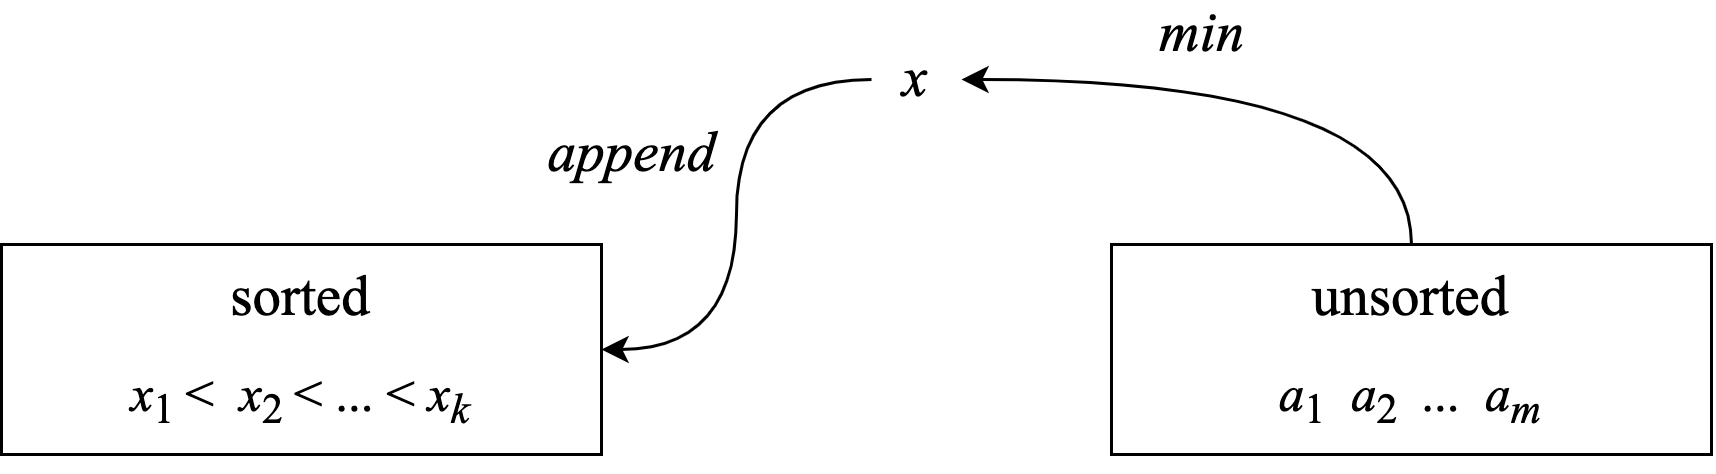
\includegraphics[scale=0.8]{img/ssort}
  \caption{The left is sorted, repeatedly select the minimum of the rest and append.}
  \label{fig:sel-sort}
\end{figure}

We can improve it to in-place sort by reusing $A$. Place the minimum in $A[1]$, the second smallest in $A[2]$, ... When find the $i$-th smallest element, swap it with $A[i]$.

\begin{algorithmic}[1]
\Function{Sort}{$A$}
  \For{$i \gets 1$ to $|A|$}
    \State $m \gets$ \Call{Min-At}{$A, i$}
    \State \textproc{Exchange} $A[i] \leftrightarrow A[m]$
  \EndFor
\EndFunction
\end{algorithmic}

Let $A = [a_1, a_2, ..., a_n]$, when select the $i$-th smallest element, $[a_1, a_2, ..., a_{i-1}]$ are sorted. Call \textproc{Min-At}($A, i$) to find the minimum of $[a_i, a_{i+1}, ..., a_n]$, then swap with $a_i$. Repeat this to process all elements as shown in \cref{fig:in-place-ssort}.

\begin{figure}[htbp]
  \centering
  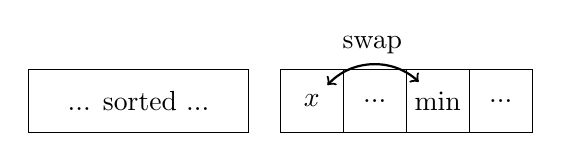
\begin{tikzpicture}[scale=0.8]
    \draw (0, 0) rectangle (3.5,1) node[pos=.5] {... sorted ...};
    \draw (4, 0) rectangle (5, 1) node (x) [pos=.5] {$x$};
    \draw (5, 0) rectangle (6, 1) node[pos=.5] {...};
    \draw (6, 0) rectangle (7, 1) node (min) [pos=.5] {$\min$};
    \draw (7, 0) rectangle (8, 1) node[pos=.5] {...};
    \draw[thick, <->] (x) edge[bend left=45] node [above] {swap} (min);
  \end{tikzpicture}
  \caption{The left is sorted, repeatedly find the minimum and swap to the right position.}
  \label{fig:in-place-ssort}
\end{figure}

\section{Find the minimum}
\index{selection sort!min}

We use the `compare and swap' method to find the minimum. Label the elements with $1, 2, ..., n$. Compare the elements of number 1 and 2, pick the smaller and compare it with number 3, ... repeat till the last element of number $n$.

\begin{algorithmic}[1]
\Function{Min-At}{$A, i$}
  \State $m \gets i$
  \For{$i \gets m + 1 $ to $|A|$}
    \If{$A[i] < A[m]$}
      \State $m \gets i$
    \EndIf
  \EndFor
  \State \Return $m$
\EndFunction
\end{algorithmic}

\index{selection sort!tail-recursive min}
\textproc{Min-At} locates the minimum at $m$ from slice $A[i...]$. $m$ starts from $A[i]$, then scan $A[i+1], A[i+2], ...$. To find the minimum of a list $L$, if $L$ is a singleton $[x]$, then $x$ is the minimum; otherwise pick an element $x$ from $L$, then recursively find the minimum $y$ from the remaining, the smaller one between $x$ and $y$ is the minimum of $L$.

\be
\begin{array}{rcl}
\min\ [x] & = & (x, [\ ]) \\
\min\ (x \cons xs) & = & \begin{cases}
  x < y: & (x, xs),\ \text{where}\ (y, ys) = \min\ xs \\
  \text{otherwise}: & (y,\ x \cons ys)
\end{cases}
\end{array}
\ee

We can further improve it to tail recursive. Divide the elements into two groups $A$ and $B$. $A$ is initialized empty ($[\ ]$), $B$ contains all elements. We pick two elements from $B$, compare and put the greater one to $A$, leave the smaller one as $m$. Then repeatedly pick element from $B$, compare with $m$ till $B$ becomes empty. $m$ holds the minimum finally. At any time, we have the invariant: $L = A \doubleplus [m] \doubleplus B$, where $a \leq m \leq b$ for every $a \in A, b \in B$.

\be
\min\ (x \cons xs) = min'\ [\ ]\ x\ xs
\ee

Where:

\be
\begin{array}{rcl}
min'\ as\ m\ [\ ] & = & (m, as) \\
min'\ as\ m\ (b \cons bs) & = & \begin{cases}
  b < m: & min'\ (m \cons as)\ b\ bs \\
  \text{otherwise}: & min'\ (b \cons as)\ m\ bs \\
\end{cases}
\end{array}
\ee

Function $\min$ returns a pair: the minimum and the list of the remaining. We define selection sort as below:

\be
\begin{array}{rcl}
sort\ [\ ] & = & [\ ] \\
sort\ xs   & = & m : (sort\ xs'),\ \text{where}\ (m, xs') = \min\ xs \\
\end{array}
\ee

\subsection{Performance}

Selection sort need scan and find the minimum for $n$ times. It compares $n + (n-1) + (n-2) + ... + 1$ times, which is $O(\dfrac{n(n+1)}{2}) = O(n^2)$. Compare to the insertion sort, selection sort performs same in the best, worst, and average cases. While insertion sort performs best at $O(n)$ (the list is in reversed ordered), and worst at $O(n^2)$.

\begin{Exercise}\label{ex:basic-sel-sort}
\Question{What is the problem with below implementation of $\min$?
\[
\begin{array}{rcl}
min'\ as\ m\ [\ ] & = & (m, as) \\
min'\ as\ m\ (b:bs) & = & \begin{cases}
  b < m: & min'\ (as \doubleplus [m])\ b\ bs \\
  \text{otherwise}: & min'\ (as \doubleplus [b])\ m\ bs \\
\end{cases}
\end{array}
\]
}
\Question{Implement the in-place selection sort.}
\end{Exercise}

\begin{Answer}[ref = {ex:basic-sel-sort}]
\Question{We should use link but not append. Appending is linear to the length of the list, while linking is constant time.}

\Question{Implement the in-place selection sort.

\begin{Bourbaki}
Void sort([K] xs) {
    var n = length(xs)
    for var i = 0 to n - 1 {
        var m = i
        for Int j = i + 1 to n - 1 {
            if xs[j] < xs[m] then m = j
        }
        swap(xs[i], xs[m])
    }
}
\end{Bourbaki}
}
\end{Answer}

\section{Improvement}

To sort in ascending, descending, and varies of ordering, we abstract the comparison as $\lhd$.

\be
\begin{array}{rcl}
sortBy \lhd\ [\ ] & = & [\ ] \\
sortBy \lhd\ xs & = & m : sortBy\ \lhd\ xs',\ \text{where}\ (m, xs') = minBy\ \lhd\ xs \\
\end{array}
\ee

We also use $\lhd$ to find the 'minimum':

\be
\begin{array}{rcl}
minBy\ \lhd\ [x] & = & (x, [\ ]) \\
minBy\ \lhd\ (x:xs) & = & \begin{cases}
  x \lhd y: & (x, xs),\ \text{where}\ (y, ys) = minBy\ xs \\
  \text{otherwise}: & (y,\ x:ys)
\end{cases}
\end{array}
\ee

\index{strict weak order}
For example, we pass the $<$ to sort a collection of numbers in ascending order: $sortBy\ (<)\ [3, 1, 4, ...]$. As the constraint, we need the comparison $\lhd$ satisfy the {\em strict weak order}\cite{wiki-sweak-order}.

\begin{itemize}
\item Irreflexivity: for all $x$, $x < x$ is false;
\item Asymmetry: for all $x$ and $y$, if $x < y$, then $y < x$ is false;
\item Transitivity, for all $x$, $y$, and $z$, if $x < y$, and $y < z$, then $x < z$.
\end{itemize}

The in-place selection sort traverses all elements, we can find the minimum as an inner loop to make the implementation compact:

\begin{algorithmic}[1]
\Procedure{Sort}{$A$}
  \For{ $i \gets 1$ to $|A|$}
    \State $m \gets i$
    \For{$j \gets i+1$ to $|A|$}
      \If{$A[i] < A[m]$}
        \State $m \gets i$
      \EndIf
    \EndFor
    \State \textproc{Exchange} $A[i] \leftrightarrow A[m]$
  \EndFor
\EndProcedure
\end{algorithmic}

After sort the first $n-1$ elements, the last one must be the maximum. We can save the last loop. Besides, we needn't swap if the $i$-th smallest is exactly $A[i]$.

\begin{algorithmic}[1]
\Procedure{Sort}{$A$}
  \For{ $i \gets 1$ to $|A|-1$}
    \State $m \gets i$
    \For{$j \gets i+1$ to $|A|$}
      \If{$A[i] < A[m]$}
        \State $m \gets i$
      \EndIf
    \EndFor
    \If{$m \neq i$}
      \State \textproc{Exchange} $A[i] \leftrightarrow A[m]$
    \EndIf
  \EndFor
\EndProcedure
\end{algorithmic}

\subsection{Cock-tail sort}
\index{Cock-tail sort}

Knuth gives another selection sort implementation\cite{TAOCP}. Select the maximum, but not the minimum, and move it to the tail, as shown in \cref{fig:knuth-ssort}. At any time, the right most part is sorted. We scan the unsorted part, find the maximum and swap to the right.

\begin{algorithmic}[1]
\Procedure{Sort'}{$A$}
  \For{ $i \gets |A|$ down-to $2$}
    \State $m \gets i$
    \For{$j \gets 1$ to $i-1$}
      \If{$A[m] < A[i]$}
        \State $m \gets i$
      \EndIf
    \EndFor
    \State \textproc{Exchange} $A[i] \leftrightarrow A[m]$
  \EndFor
\EndProcedure
\end{algorithmic}

\begin{figure}[htbp]
  \centering
  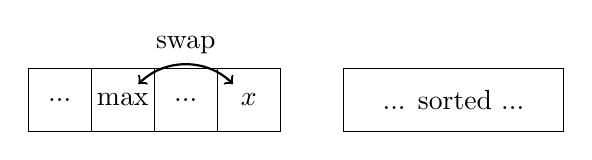
\begin{tikzpicture}[scale=0.8]
    \draw (5, 0) rectangle (6, 1) node[pos=.5] {...};
    \draw (6, 0) rectangle (7, 1) node (max) [pos=.5] {$\max$};
    \draw (7, 0) rectangle (8, 1) node[pos=.5] {...};
    \draw (8, 0) rectangle (9, 1) node (x) [pos=.5] {$x$};
    \draw (10,0) rectangle (13.5,1) node[pos=.5] {... sorted ...};
    \draw[thick, <->] (x) edge[bend right=45] node [above] {swap} (max);
  \end{tikzpicture}
  \caption{Select the maximum and swap to tail}
  \label{fig:knuth-ssort}
\end{figure}

We obtain the ascending order as well. Further, we can pick both the minimum and maximum in one pass, swap the minimum to the head, and the maximum to the tail. We can halve the inner loop times. The method is called `cock-tail sort'.

\begin{algorithmic}[1]
\Procedure{Sort}{$A$}
  \For{$i \gets 1 $ to $\lfloor \dfrac{|A|}{2} \rfloor$}
    \State $min \gets i$
    \State $max \gets |A| + 1 - i$
    \If{$A[max] < A[min]$}
      \State \textproc{Exchange} $A[min] \leftrightarrow A[max]$
    \EndIf
    \For{$j \gets i + 1$ to $|A| - i$}
      \If{$A[j] < A[min]$}
        \State $min \gets j$
      \EndIf
      \If{$A[max] < A[j]$}
        \State $max \gets j$
      \EndIf
    \EndFor
    \State \textproc{Exchange} $A[i] \leftrightarrow A[min]$
    \State \textproc{Exchange} $A[|A|+1-i] \leftrightarrow A[max]$
  \EndFor
\EndProcedure
\end{algorithmic}

\begin{figure}[htbp]
  \centering
  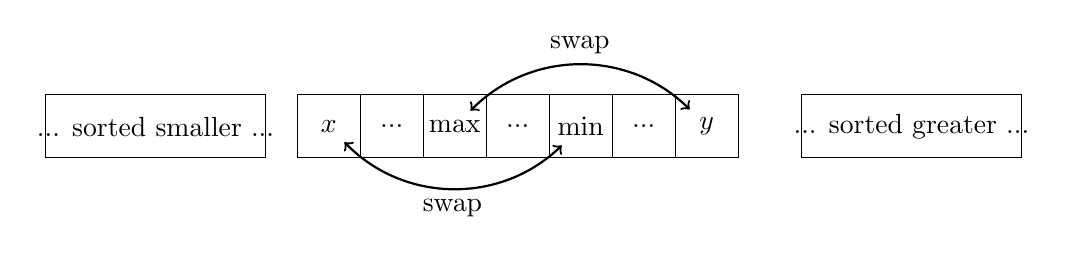
\begin{tikzpicture}[scale=0.8]
    \draw (0,0) rectangle (3.5,1) node[pos=.5] {... sorted smaller ...};
    \draw (4, 0) rectangle (5, 1) node (x) [pos=.5] {$x$};
    \draw (5, 0) rectangle (6, 1) node[pos=.5] {...};
    \draw (6, 0) rectangle (7, 1) node (max) [pos=.5] {$\max$};
    \draw (7, 0) rectangle (8, 1) node[pos=.5] {...};
    \draw (8, 0) rectangle (9, 1) node (min) [pos=.5] {$\min$};
    \draw (9, 0) rectangle (10, 1) node[pos=.5] {...};
    \draw (10, 0) rectangle (11, 1) node (y) [pos=.5] {$y$};
    \draw (12,0) rectangle (15.5,1) node[pos=.5] {... sorted greater ...};
    \draw[thick, <->] (x) edge[bend right=45] node [below] {swap} (min);
    \draw[thick, <->] (y) edge[bend right=45] node [above] {swap} (max);
  \end{tikzpicture}
  \caption{Find the minimum and maximum, swap both to the right positions.}
  \label{fig:cock-tail-sort}
\end{figure}

It's necessary to swap if the right most element less than the right most one before the inner loop. This is because the scan excludes them. We can also implement the cock-tail sort recursively:

\begin{enumerate}
  \item If the list is empty or singleton, it's sorted;
  \item Otherwise, we select the minimum and the maximum, move them  to the head and tail, then recursively sort the rest elements.
\end{enumerate}

\be
\begin{array}{rcl}
sort\ [\ ] & = & [\ ] \\
sort\ [x] & = & [x] \\
sort\ xs & = & a : (sort\ xs') \doubleplus [b], \text{where}\ (a, b, xs') = \textit{minMax}\ xs \\
\end{array}
\ee

Where function \textit{minMax} extracts the minimum and maximum from a list:

\be
\textit{minMax}\ (x:y:xs) = foldr\ sel (\min\ x\ y, \max\ x\ y, [\ ])\ xs
\ee

We initialize the minimum as the first element $x_0$, and the maximum as the second element $x_1$, and process the list with $foldr$. Function $sel$ is defined as:

\[
sel\ x\ (x_0, x_1, xs) = \begin{cases}
  x < x_0: & (x, x_1, x_0 : xs) \\
  x_1 < x: & (x_0, x, x_1 : xs) \\
  \text{otherwsie}: & (x_0, x_1, x : xs) \\
\end{cases}
\]

Although \textit{minMax} is bound to $O(n)$ time, $\doubleplus[b]$ is expensive. As shown in \cref{fig:cock-tail-sort}, let the left sorted part be $A$, the right sorted part be $B$. We can turn the cock-tail sort to tail recursive with $A$ and $B$ as the accumulators.

\be
\begin{array}{rcl}
sort'\ A\ B\ [\ ] & = & A \doubleplus B \\
sort'\ A\ B\ [x]  & = & A \doubleplus (x:B) \\
sort'\ A\ B\ (x:xs) & = & sort'\ (A \doubleplus [x_0])\ xs'\ (x_1:B) \\
\end{array}
\ee

Where $(x_0, x_1, xs') = \textit{minMax}\ xs$. We pass empty $A$ and $B$ to initialize sorting: $sort = sort'\ [\ ]\ [\ ]$. The append only happens to $A \doubleplus [x_0]$, while $x_1$ is linked before $B$. Every recursion performs an append operation. To eliminate it, we can maintain $A$ in reversed order: $\overleftarrow{A}$, hence $x_0$ is linked ahead but appended. We have the following equations:

\be
\begin{array}{rcl}
A' & = & A \doubleplus [x] \\
   & = & reverse\ (x : reverse\ A) \\
   & = & reverse\ (x : \overleftarrow{A}) \\
   & = & \overleftarrow{ x : \overleftarrow{A}}
\end{array}
\ee

Finally, we reverse $\overleftarrow{A'}$ back to $A'$. We can improve the algorithm as below:

\be
\begin{array}{rcl}
sort'\ A\ B\ [\ ] & = & (reverse\ A) \doubleplus B \\
sort'\ A\ B\ [x]  & = & (reverse\ x:A) \doubleplus B \\
sort'\ A\ B\ (x:xs) & = & sort'\ (x_0:A)\ xs'\ (x_1:B) \\
\end{array}
\ee

\section{Further improvement}

Although cock-tail sort halves the loops, it's still bound to $O(n^2)$ time. To sort by comparison, we need the outer loop to examine all the elements for ordering. Do we need scan all the elements to select the minimum every time? After find the first smallest one, we've traversed the whole collection, obtain some information, like which are greater, which are smaller. However, we discard such information for further selection, but restart a fresh scan. The idea is information reusing. Let's see one inspired from football match.

\subsection{Tournament knock out}
\index{Tournament knock out}

The football world cup is held every four years. There are 32 teams from different continent play the final games. Before 1982, there were 16 teams in the finals. Let's go back to 1978 and imagine a special way to determine the champion: In the first round, the teams
are grouped into 8 pairs to play. There will be 8 winners, and 8 teams will be out. Then in the second round, 8 teams are grouped into 4 pairs. There will be 4 winners. Then the top 4 teams are grouped into 2 pairs, there will be two teams left for the final. The champion is determined after 4 rounds of games. There are total $8 + 4 + 2 + 1 = 15$ games. Besides the champion, we also want to know which is the silver medal team. In the real world cup, the team lost the final is the runner-up. However, it isn't fair in some sense. We often hear about the `group of death'. Suppose Brazil is grouped with Germam in round one. Although both teams are strong, one team is knocked out. It's quite possible that team would beat other teams except for the champion, as shown in \cref{fig:tournament-tree-1}.

\begin{figure}[htbp]
  \centering
  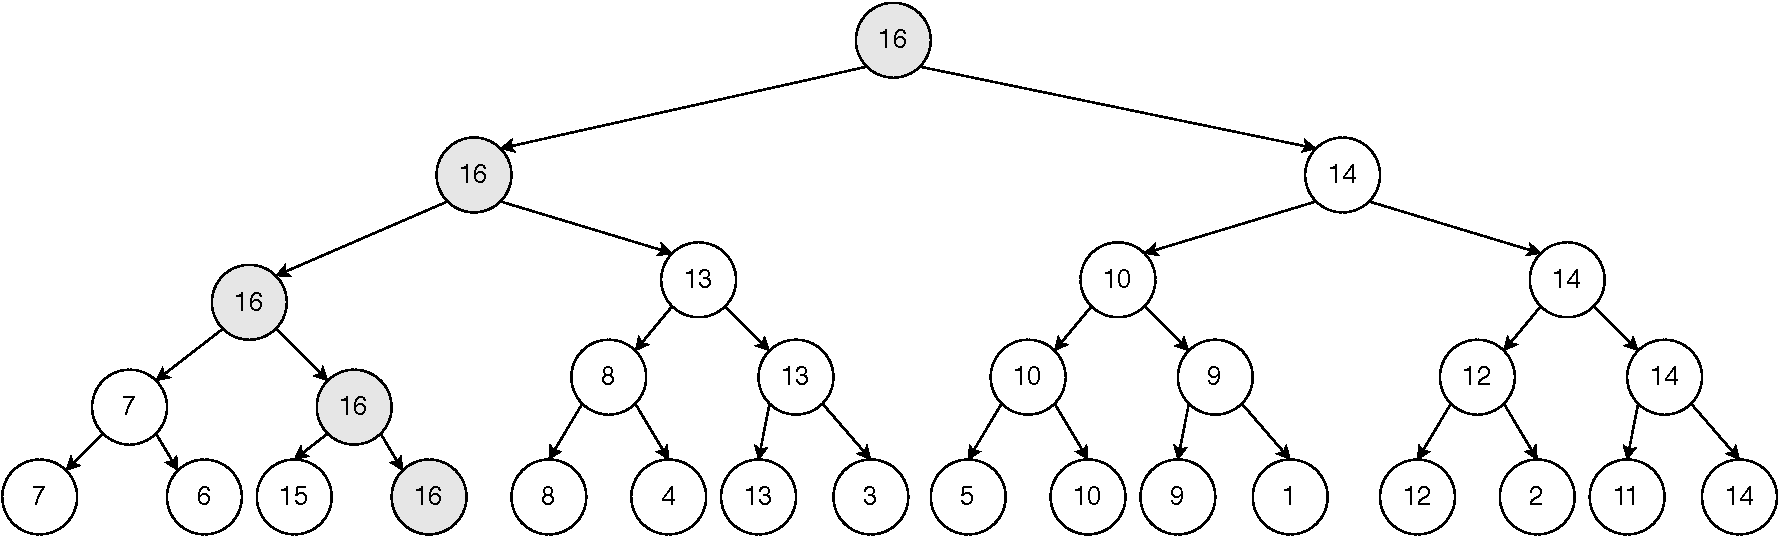
\includegraphics[scale=0.4]{img/tournament-tree-1}
  \caption{The element 15 is knocked out in the first round.}
  \label{fig:tournament-tree-1}
\end{figure}

Assign every team a number to measure its strength. Suppose the team with greater number always beats the smaller one (this is obviously not true in real world). The champion number is 16. the runner-up is not 14, but 15, which is out in the first round. We need figure out a way to quickly identify the second greater number in the tournament tree. The apply it to select the 3rd, the 4th, ... to sort. We can mutate the champion to a very small number, i.e. $-\infty$, hence it won't be selected next time, and the previous runner-up will become the new champion. For $2^m$ teams, where $m$ is some natural number, it takes $2^{m-1} + 2^{m-2} + ... + 2 + 1 = 2^m - 1$ comparisons to determine the new champion. This is same as before. Actually, we needn't perform bottom-up comparisons because the tournament tree
stores sufficient ordering information. The champion must beat the runner-up at sometime. We can locate the runner-up along the path from the root to the leaf of the champion. We grey the path in \cref{fig:tournament-tree-1} of $[14, 13, 7, 15]$. This method is defined as below:

\begin{enumerate}
\item Build a tournament tree with the maximum (the champion) at the root;
\item Take the root, replace it with $-\infty$ along the path to leaf;
\item Perform a bottom-up back-track along the path, find the new champion and store it in the root;
\item Repeat step 2 to process all elements.
\end{enumerate}

\captionsetup[subfigure]{labelformat=empty, margin=10pt}
\begin{figure}[htbp]
  \centering
  \subcaptionbox{Take 16, replace with $-\infty$, 15 becomes the new root.}{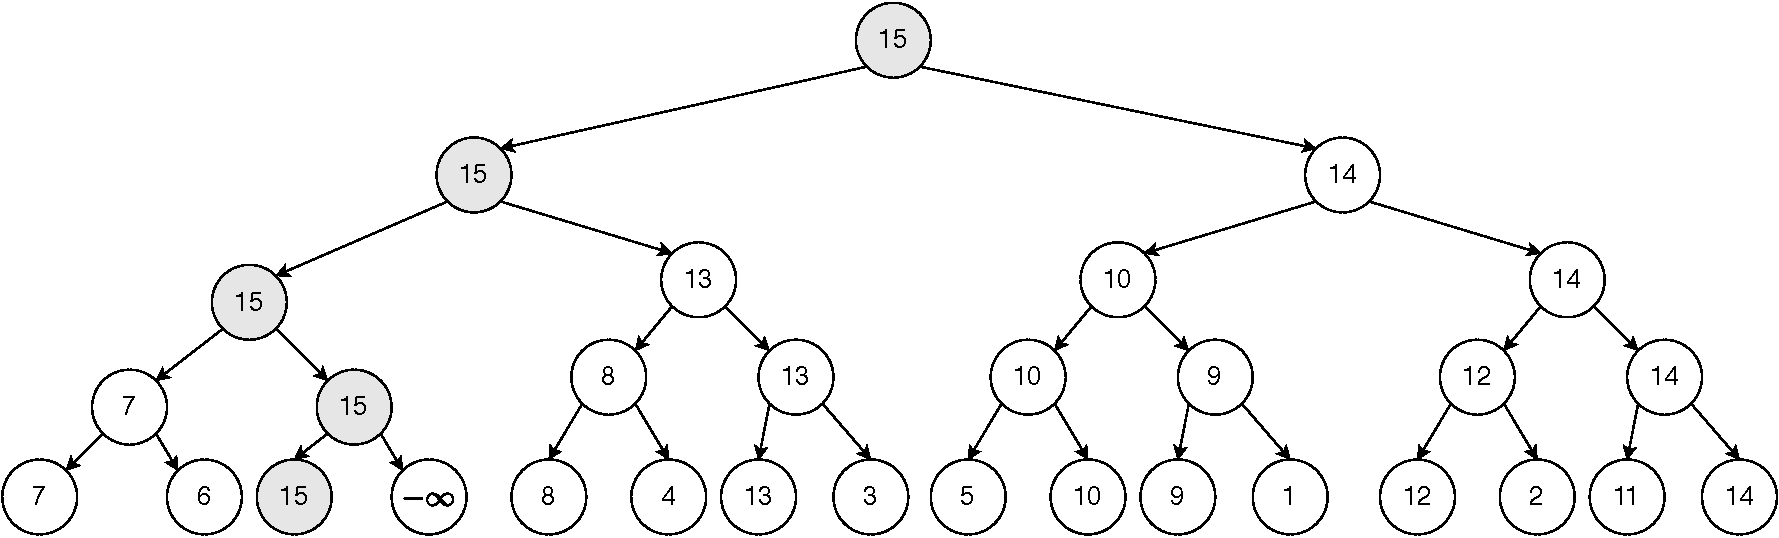
\includegraphics[scale=0.4]{img/tournament-tree-2}} \\
  \subcaptionbox{Take 15, replace with $-\infty$, 14 becomes the new root.}{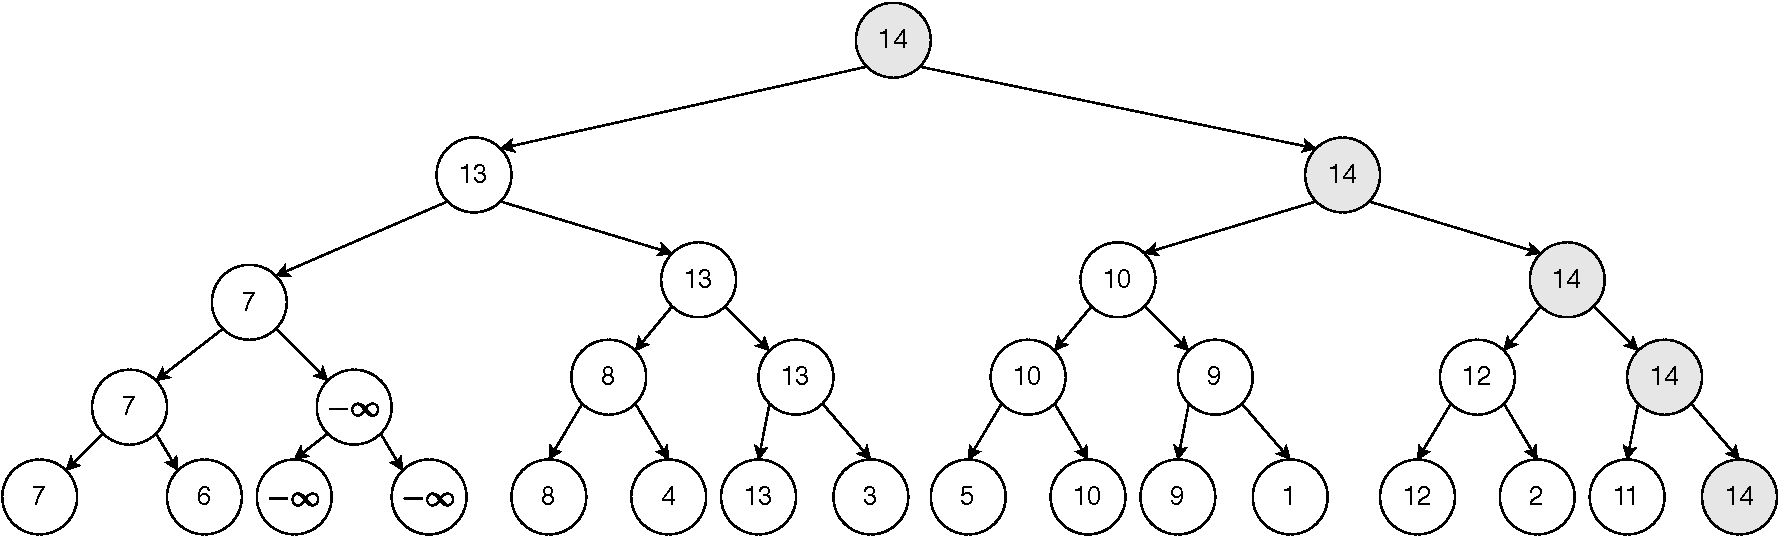
\includegraphics[scale=0.4]{img/tournament-tree-3}} \\
  \subcaptionbox{Take 14, replace with $-\infty$, 13 becomes the new root.}{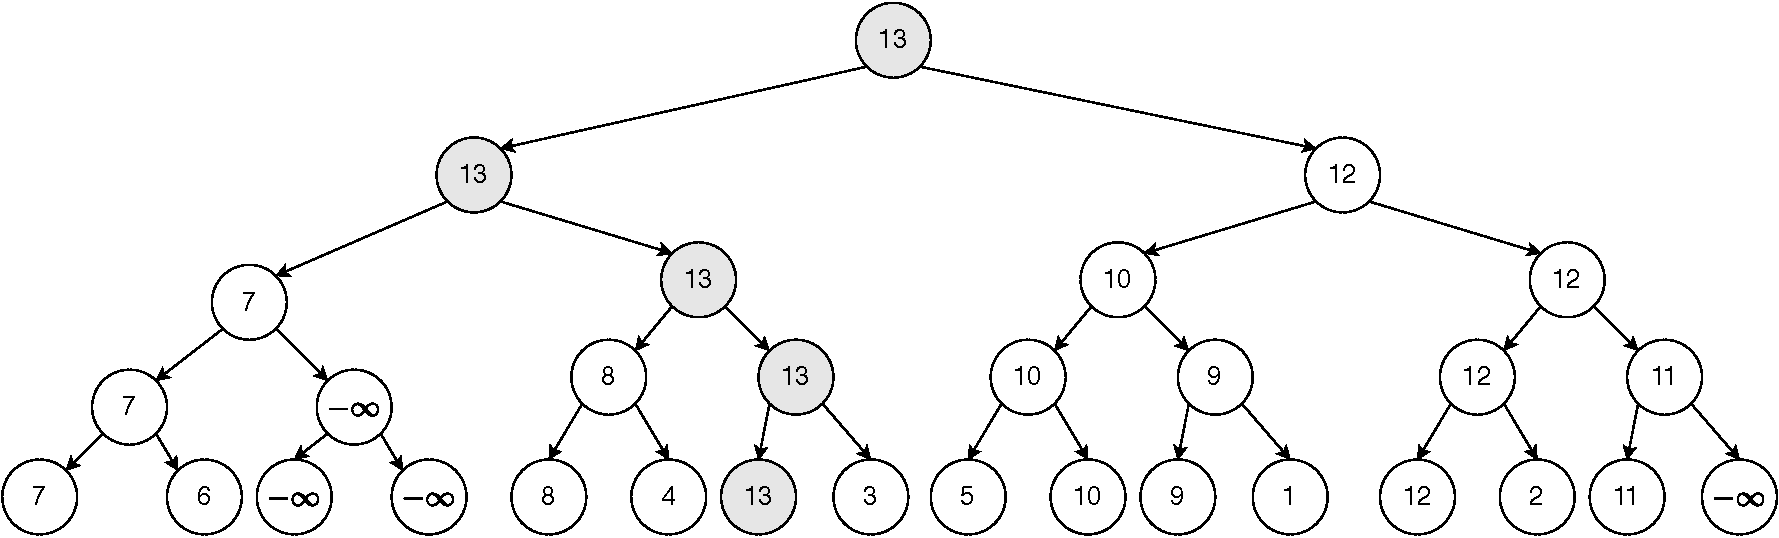
\includegraphics[scale=0.4]{img/tournament-tree-4}}
  \caption{The first 3 steps of tournament tree sort.}
  \label{fig:tournament-tree-4}
\end{figure}
\captionsetup[subfigure]{labelformat=parens}

To sort a collection of elements, we build a tournament tree from them, repeatedly select the champion from it. \Cref{fig:tournament-tree-4} gives the first 3 steps. We can re-use the binary tree definition. To make back-track easy, we need the parent field in each node. When $n$ is not $2^m$ form some natural number $m$, there is remaining element without ``player'', and directly enters the next round of games. To build the tournament tree, we build $n$ singleton trees from every element. Then pick every two $t_1$, $t_2$ to create a bigger binary tree $t$. Where the root of $t$ is $\max(key(t_1), key(t_2))$, the left and right sub-trees are $t_1$, $t_2$. Repeat to obtain a collection of new trees, each height increases by one. If there is remaining, then enters the next round. After this round, trees halve to $\lfloor \dfrac{n}{2} \rfloor$. Repeat this to obtain the final tournament tree. The process is bound to $O(n + \dfrac{n}{2} + \dfrac{n}{4} + ... ) = O(2n) = O(n)$ time.

\begin{algorithmic}[1]
\Function{Build-Tree}{$A$}
  \State $T \gets [\ ]$
  \For{each $x \in A$}
    \State \textproc{Append}($T$, \Call{Node}{NIL, $x$, NIL})
  \EndFor
  \While{$|T| > 1$}
    \State $T' \gets [\ ]$
    \For{every $t_1, t_2 \in T$}
      \State $k \gets$ \textproc{Max}(\Call{Key}{$t_1$}, \Call{Key}{$t_2$})
      \State \textproc{Append}($T'$, \Call{Node}{$t_1$, $k$, $t_2$})
    \EndFor
    \If{|T| is odd}
      \State \textproc{Append}($T'$, \Call{Last}{$T$})
    \EndIf
    \State $T \gets T'$
  \EndWhile
  \State \Return $T[1]$
\EndFunction
\end{algorithmic}

We replace the root with $-\infty$ top-down, then back-track through the parent field to find the new maximum.

\begin{algorithmic}[1]
\Function{Pop}{$T$}
  \State $m \gets$ \Call{Key}{$T$}
  \State \Call{Key}{$T$} $\gets -\infty$
  \While{$T$ is not leaf}  \Comment{top-down replace $m$ with $-\infty$.}
    \If{\textproc{Key}(\Call{Left}{$T$}) $ = m$}
      \State $T \gets$ \Call{Left}{$T$}
    \Else
      \State $T \gets$ \Call{Right}{$T$}
    \EndIf
    \State \Call{Key}{$T$} $\gets -\infty$
  \EndWhile
  \While{\Call{Parent}{$T$} $\neq$ NIL} \Comment{bottom-up to find the new maximum.}
    \State $T \gets$ \Call{Parent}{$T$}
    \State \Call{Key}{$T$} $\gets$ \textproc{Max}(\textproc{Key}(\Call{Left}{$T$}), \textproc{Key}(\Call{Right}{$T$}))
  \EndWhile
  \State \Return $(m, T)$ \Comment{the maximum and the new tree.}
\EndFunction
\end{algorithmic}

\textproc{Pop} process the tree in two passes, top-down, then bottom-up along the path of the champion. Because the tournament tree is balanced, the length of this path, i.e. height of the tree, is bound to $O(\lg n)$, where $n$ is the number of the elements. Below is the tournament tree sort. We first build the tree in $O(n)$ time, then pop the maximum for $n$ times, each pop takes $O(\lg n)$ time. The total time is bound to $O(n \lg n)$.

\begin{algorithmic}
\Procedure{Sort}{$A$}
  \State $T \gets$ \Call{Build-Tree}{$A$}
  \For{$i \gets |A|$ down to $1$}
    \State $A[i] \gets$ \Call{Extract-Max}{$T$}
  \EndFor
\EndProcedure
\end{algorithmic}

We can also implement tournament tree sort recursively. Reuse the binary search tree definition, let an none empty tree be $(l, k, r)$, where $k$ is the element, $l$, $r$ are the left and right sub-trees. Define $wrap\ x = (\nil, x, \nil)$ to create a leaf node. We can convert the $n$ elements to a list of $n$ single trees: $ts = map\ wrap\ xs$. For every pair of trees $t_1$, $t_2$, we merge them to a bigger tree, pick the greater element as the new root, and $t_1$, $t_2$ become the left and right sub-trees.

\be
merge\ t_1\ t_2 = (t_1, \max\ k_1\ k_2, t_2)
\ee

Where $k_1 = key\ t_1, k_2 = key\ t_2$ are the elements at root respectively. Define a function $build\ ts$ to repeatedly merge two trees, and build the final tournament tree.

\be
\begin{array}{rcl}
build\ [\ ] & = & \nil \\
build\ [t]  & = & t \\
build\ ts & = & build\ (\textit{pairs}\ ts) \\
\end{array}
\ee

Where:

\be
\begin{array}{rcl}
\textit{pairs}\ (t_1:t_2:ts) & = & (merge\ t_1\ t_2) : \textit{pairs}\ ts \\
\textit{pairs}\ ts & = & ts \\
\end{array}
\ee

When pop the champion, we examine the sub-trees to see which one holds the same element as the root. Then recursively pop the champion from the sub-tree till the leaf node. Then replace it with $-\infty$.

\be
\begin{array}{rcl}
pop\ (\nil, k, \nil) & = & (\nil, -\infty, \nil) \\
pop\ (l, k, r) & = & \begin{cases}
  k = key\ l: & (l', \max\ (key\ l')\ (key\ r), r), \text{where} l' = pop\ l \\
  k = key\ r: & (l,  \max\ (key\ l)\ (key\ r'), r'), \text{where} r' = pop\ r \\
\end{cases}
\end{array}
\ee

Then repeatedly pop from the tournament tree to sort (in descending order):

\be
\begin{array}{rcl}
sort\ \nil & = & [\ ] \\
sort\ (l, -\infty, r) & = & [\ ]  \\
sort\ t & = & (key\ t) : sort\ (pop\ t) \\
\end{array}
\label{eq:tsort}
\ee

\begin{Exercise}\label{ex:tournament-tree-sort}
\Question{Implement the recursive tournament tree sort in ascending order.}\label{ex:parameterized-tournament-tree-sort}
\Question{How to handle duplicated element with the tournament tree? is tournament tree sort stable?}
\Question{Compare the tournament tree sort and binary search tree sort in terms of space and time performance.}
\Question{Compare heap sort and tournament tree sort in terms of space and time performance.}
\end{Exercise}

\begin{Answer}[ref = {ex:tournament-tree-sort}]
\Question{Implement the recursive tournament tree sort in ascending order.

We can realize the ascending sort by replacing the $max$ and $-\infty$ with the $min$ and $\infty$. Further, we can abstract them as two parameters:

\begin{Haskell}
minBy p a b = if p a b then a else b

merge p t1 t2 = Br t1 (minBy p (key t1) (key t2)) t2

fromListWith p xs = build $ map wrap xs where
  build [] = Empty
  build [t] = t
  build ts = build $ pair ts
  pair (t1:t2:ts) = (merge p t1 t2) : pair ts
  pair ts = ts

popWith p inf = delMin where
  delMin (Br Empty _ Empty) = Br Empty inf Empty
  delMin (Br l k r) | k == key l = let l' = delMin l in
                      Br l' (minBy p (key l') (key r)) r
                    | k == key r = let r' = delMin r in
                      Br l (minBy p (key l) (key r')) r'

toListWith p inf = flat where
  flat Empty = []
  flat t | inf == key t = []
         | otherwise = (top t) : (flat $ popWith p inf t)

sortBy p inf xs = toListWith p inf $ fromListWith p xs where
\end{Haskell}

$sortBy\ (<)\ \infty$ defines the ascending sort, and $sortBy\ (>)\ -\infty$ defines the descending sort.
}

\Question{How to handle duplicated element with the tournament tree? is tournament tree sort stable?

From \cref{ex:parameterized-tournament-tree-sort}, we can handle the duplicated elements with $sortBy\ (\leq)\ \infty$ (ascending sort) for example. The tournament tree sort is not stable.
}

\Question{Compare the tournament tree sort and binary search tree sort in terms of space and time performance.

They are both bound to $O(n \lg n)$ time, and $O(n)$ space. The difference is, the binary search tree does not change after build (unless insert, delete), while the tournament tree changes to a tree with $n$ nodes of infinity.
}

\Question{Compare heap sort and tournament tree sort in terms of space and time performance.

They are both bound to $O(n \lg n)$ time, and $O(n)$ space. The difference is, the heap becomes empty after sort complete, while the tournament tree still occupies $O(n)$ space.
}
\end{Answer}

\subsection{Heap sort}

We improve the selection based sort to $O(n \lg n)$ time through tournament tree. It is the upper limit of the comparison based sort\cite{TAOCP}. However, there are still rooms for improvement. After sort, The binary holds all $-\infty$, occupying $2n$ nodes for $n$ elements. It's there a way to release node after pop? Can we halve $2n$ nodes to $n$? Treat the tree as empty when the root element is $-\infty$, and rename $key$ to $top$, we can write \cref{eq:tsort} in a generic way:

\be
\begin{array}{rcl}
sort\ \nil & = & [\ ] \\
sort\ t & = & (top\ t) : sort\ (pop\ t) \\
\end{array}
\ee

This is exactly as same as the definition of heap sort. Heap always stores the minimum (or the maximum) on the top, and provides fast pop operation. The array implementation encodes the binary tree structure as indices, uses exactly $n$ cells to represent the heap. The functional heaps, like the leftist heap and splay heap use $n$ nodes as well. We'll give more well performed heaps in next chapter.

\section{Appendix - example programs}

Tail recursive selection sort:
\begin{Haskell}
sort [] = []
sort xs = x : sort xs'
  where
    (x, xs') = extractMin xs

extractMin (x:xs) = min' [] x xs
  where
    min' ys m [] = (m, ys)
    min' ys m (x:xs) = if m < x then min' (x:ys) m xs
                                else min' (m:ys) x xs
\end{Haskell}

Cock-tail sort:

\begin{lstlisting}[language = Bourbaki]
[A] cocktailSort([A] xs) {
    Int n = length(xs)
    for Int i = 0 to n / 2 {
        var (mi, ma) = (i, n - 1 -i)
        if xs[ma] < xs[mi] then swap(xs[mi], xs[ma])
        for Int j = i + 1 to n - 1 - i {
            if xs[j] < xs[mi] then mi = j
            if xs[ma] < xs[j] then ma = j
        }
        swap(xs[i], xs[mi])
        swap(xs[n - 1 - i], xs[ma])
    }
    return xs
}
\end{lstlisting}

Tail recursive cock-tail sort:

\begin{Haskell}
csort xs = cocktail [] [] xs
  where
    cocktail as bs []  = reverse as ++ bs
    cocktail as bs [x] = reverse (x:as) ++ bs
    cocktail as bs xs  = let (mi, ma, xs') = minMax xs
                         in cocktail (mi:as) (ma:bs) xs'

minMax (x:y:xs) = foldr sel (min x y, max x y, []) xs
  where
    sel x (mi, ma, ys) | x < mi = (x, ma, mi:ys)
                       | ma < x = (mi, x, ma:ys)
                       | otherwise = (mi, ma, x:ys)
\end{Haskell}

Build the tournament tree (reuse the binary tree structure):

\begin{lstlisting}[language = Bourbaki]
Node<T> build([T] xs) {
    [T] ts = []
    for x in xs {
        append(ts, Node(null, x, null))
    }
    while length(ts) >  1 {
        [T] ts' = []
        for l, r in ts {
            append(ts', Node(l, max(l.key, r.key), r))
        }
        if odd(length(ts)) then append(ts', last(ts))
        ts = ts'
    }
    return ts[0];
}
\end{lstlisting}

Pop from the tournament tree:

\begin{lstlisting}[language = Bourbaki]
T pop(Node<T> t) {
    T m = t.key
    t.key = -INF
    while not isLeaf(t) {
        t = if t.left.key == m then t->left else t->right
        t.key = -INF
    }
    while (t.parent != null) {
        t = t.parent
        t.key = max(t.left.key, t.right.key)
    }
    return (m, t);
}
\end{lstlisting}

Tournament tree sort:

\begin{lstlisting}[language = Bourbaki]
void sort([A] xs) {
    Node<T> t = build(xs)
    for Int n = length(xs) - 1 downto 0 {
        (xs[n], t) = pop(t)
    }
}
\end{lstlisting}

Recursive tournament tree sort (descending order):

\begin{Haskell}
data Tr a = Empty | Br (Tr a) a (Tr a)

data Infinite a = NegInf | Only a | Inf deriving (Eq, Ord)

key (Br _ k _ ) = k

wrap x = Br Empty (Only x) Empty

merge t1@(Br _ k1 _) t2@(Br _ k2 _) = Br t1 (max k1 k2) t2

fromList = build . (map wrap) where
  build [] = Empty
  build [t] = t
  build ts = build (pairs ts)
  pairs (t1:t2:ts) = (merge t1 t2) : pair ts
  pairs ts = ts

pop (Br Empty _ Empty) = Br Empty NegInf Empty
pop (Br l k r) | k == key l = let l' = pop l in Br l' (max (key l') (key r)) r
               | k == key r = let r' = pop r in Br l (max (key l) (key r')) r'

toList Empty = []
toList (Br _ Inf _) = []
toList t@(Br _ Only k _) = k : toList (pop t)

sort = toList . fromList
\end{Haskell}

\ifx\wholebook\relax\else
\section{Answer}
\shipoutAnswer

\begin{thebibliography}{99}

\bibitem{TAOCP}
Donald E. Knuth. ``The Art of Computer Programming, Volume 3: Sorting and Searching (2nd Edition)''. Addison-Wesley Professional; 2 edition (May 4, 1998) ISBN-10: 0201896850 ISBN-13: 978-0201896855

\bibitem{CLRS}
Thomas H. Cormen, Charles E. Leiserson, Ronald L. Rivest and Clifford Stein.
``Introduction to Algorithms, Second Edition''. ISBN:0262032937. The MIT Press. 2001

\bibitem{wiki-sweak-order}
Wikipedia. ``Strict weak order''. \url{https://en.wikipedia.org/wiki/Strict_weak_order}

\end{thebibliography}

\expandafter\enddocument
\fi
